\documentclass[]{article}
\usepackage[T1]{fontenc}
\usepackage[top=1in, bottom=1in, left=1in, right=1in]{geometry}
\usepackage{commath,amsmath,amssymb,amsfonts}
\usepackage{newtxtext, newtxmath}
\usepackage{float}
\usepackage{algorithmic}
\usepackage{graphicx}
\graphicspath{{./images/}}
\usepackage{textcomp}
\usepackage{xcolor}
\usepackage[backend=biber, sorting=none]{biblatex}
\usepackage[hidelinks]{hyperref}

%uncomment below line to use reference file
%\addbibresource{references.bib}

%opening
\title{VR Report}
\author{Benjamin Russell - fdmw97}
\date{}

\begin{document}

\maketitle

\section{Static Renders}
Presented below are static renders demonstrating the inverse Lateral Chromatic Aberration (LCA) correction, fragment shader based pre-distortion, and mesh based pre-distortion.
\begin{figure}[h!]
	\centering
	\begin{minipage}[H]{0.2\textwidth}
		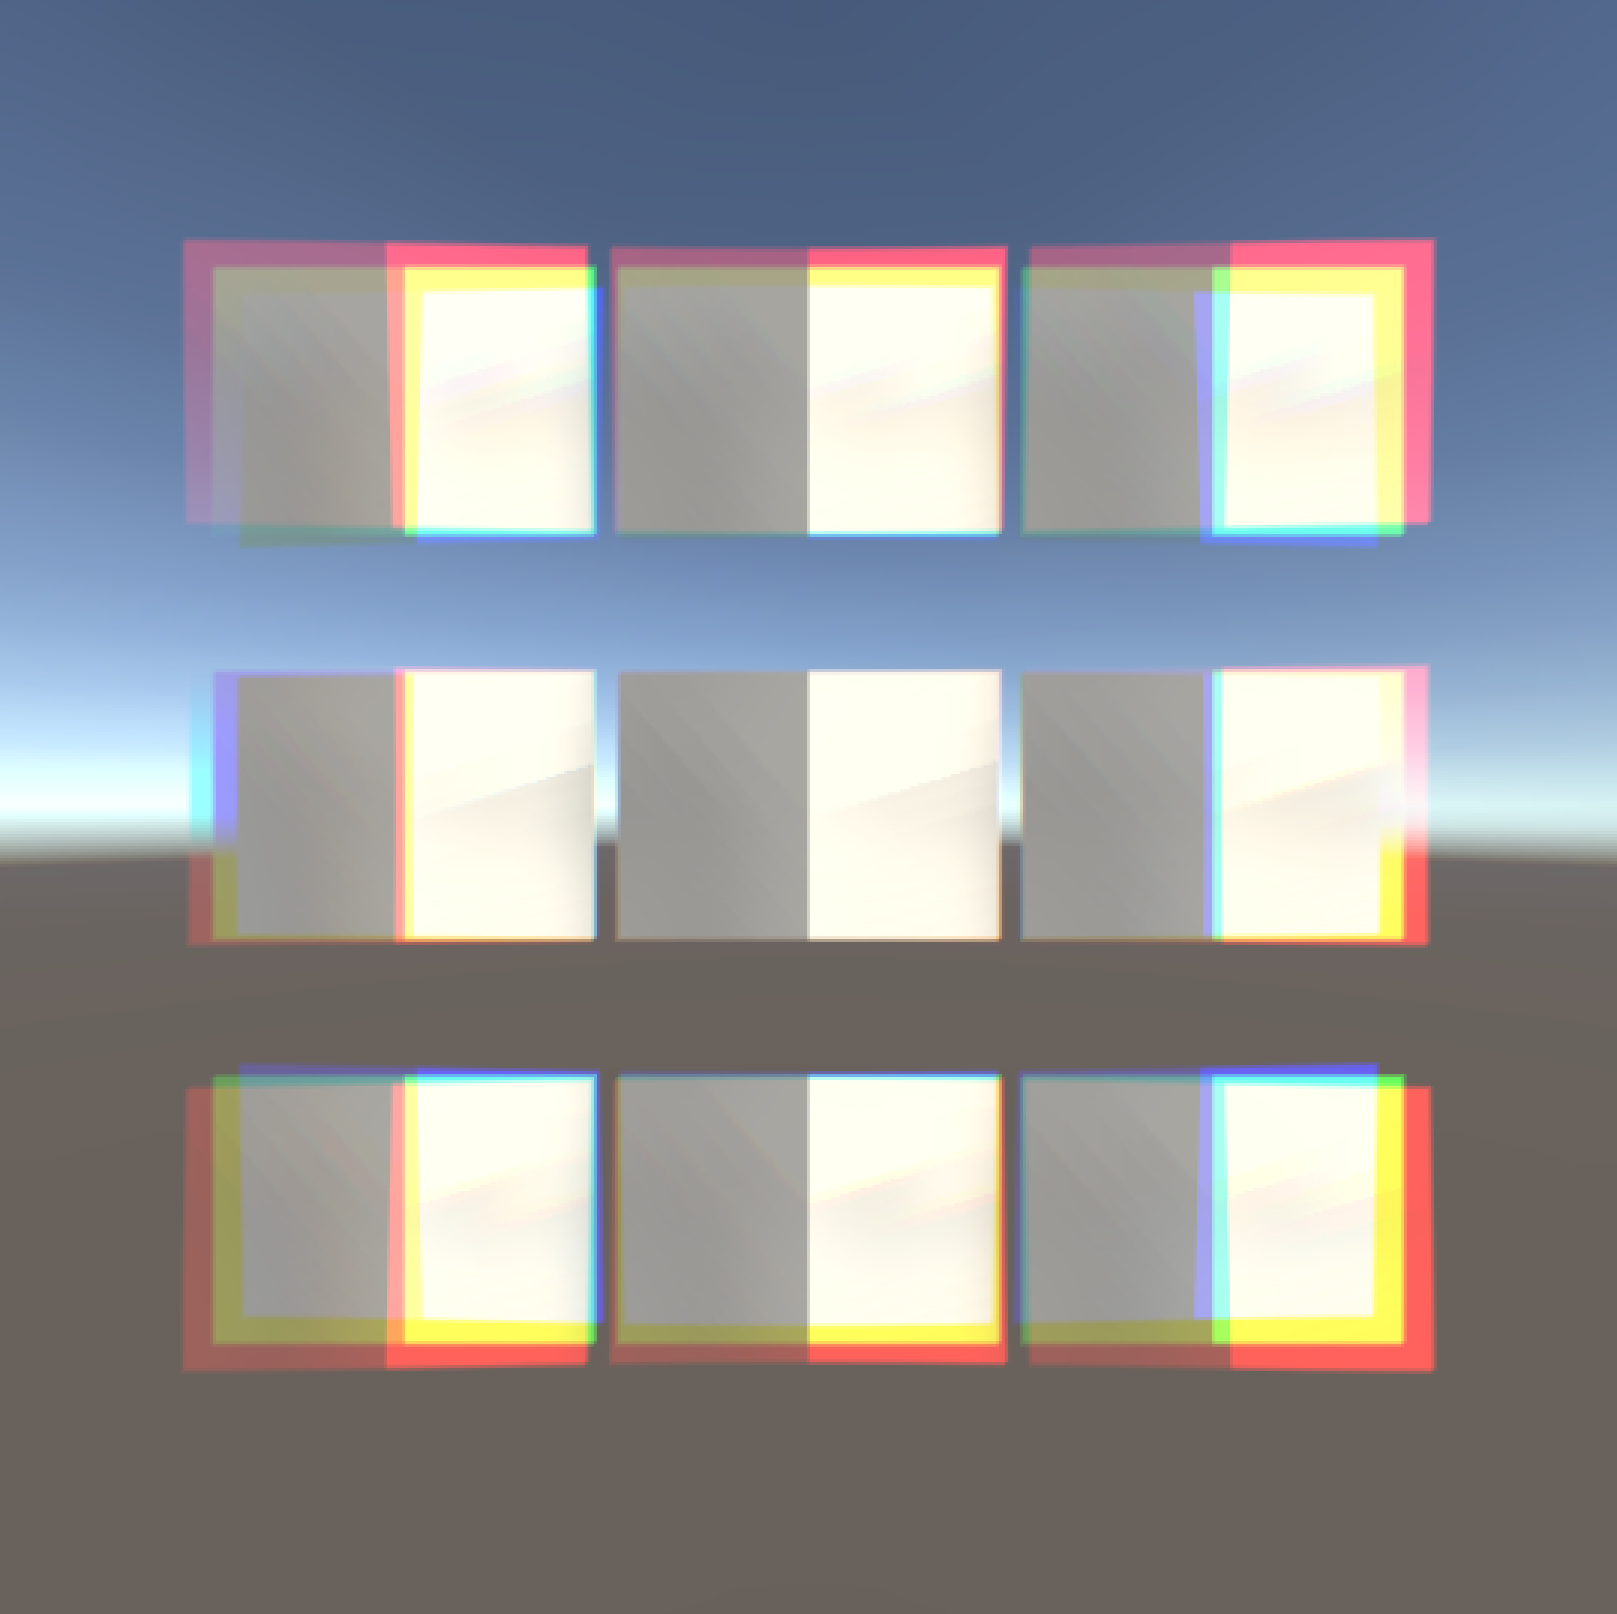
\includegraphics[width=4cm]{LCA_45}
		\caption{Static render of cubes at 45 degrees using inverse LCA correction}
		\label{fig:lca_45}
	\end{minipage}
	\hfill
	\begin{minipage}[H]{0.2\textwidth}
		
\includegraphics[width=4cm]{Barrel_Frag_45}
		\caption{Static render of cubes at 45 degrees using fragment shader based pre-distortion}
		\label{fig:frag_45}
	\end{minipage}
	\hfill
	\begin{minipage}[H!]{0.2\textwidth}
		
\includegraphics[width=4cm]{Barrel_Vec_45}
		\caption{Static render of cubes at 45 degrees using mesh based pre-distortion with 512 triangle mesh}
		\label{fig:vec_45}
	\end{minipage}
\end{figure}

\section{Comparison of Pixel and Mesh Based Pre-Distortion}
Pixel based pre-distortion has the advantage of being much easier to implement that mesh based pre-distortion as it is simply sampling each pixel from the texture at its new distorted radius. When compared to a mesh based method with a low vertex/triangle count the pixel based method produces far more accurate results as the accuracy is as good as the textures resolution which can be made very high quite easily. This is shown in \autoref{fig:res_mesh_comp} where it is clear that the since the texture/frame-buffer resolution is greater than the vertex/triangle count of the mesh the pixel based pre-distortion is more accurate, with the low vertex mesh based method showing hard edges and other distortions on the outer cubes rather than the smooth curved barrel distorted edges in the pixel based method.
\begin{figure}[H]
	\centering
	\begin{minipage}[H]{0.2\textwidth}
		
\includegraphics[width=4cm]{Barrel_Frag_45}
	\end{minipage}
	\hspace{1cm}
	\begin{minipage}[H]{0.2\textwidth}
		
\includegraphics[width=4cm]{Barrel_Vec_32}
	\end{minipage}
	\caption{Comparison of pixel based pre-distortion 512x512 resolution (left) and mesh based pre-distortion 32 triangle mesh (right)}
	\label{fig:res_mesh_comp}
\end{figure}
The advantage of using a the mesh based method is in the number of required calculations in the shader. When using the pixel based method the distorted radius is calculated on a per pixel basis which in the case of the 512x512 render texture used in this project is 262,144 distortion calculations. When compared to using a mesh of just 128 triangles/81 vertices which only requires distorting the individual vertices so 81 distortion calculations, the actual distortion of the image using the mesh based method leverages the interpolation that takes place between the fragment and vertex shader in order to save on direct computation of distortion for each pixel as these values are interpolated based on the vertex distortions instead. The number of texture lookups in both methods is determined by the output resolution of the scene as we have to sample the texture for each fragment to determine the final colour on the screen. Even though the computational cost is reduced by using the mesh based method to calculate where to sample the texture (thanks to interpolation), it is still necessary to sample the texture for the same number of fragments as the pixel based method.
\subsection{Effect Of Vertex Count On Mesh Based Pre-Distortion}



%uncomment below line to print bilbliography
%\printbibliography
\end{document}
